\subsection{Modulo UART}
\label{sec:UART}
	Si consideramos la lista de elementos dinámicos y cada estado que pueden admitir, es claro que la cantidad de señales sobrepasaría por mucho la limitada cantidad de puertos que una FPGA pueda proveer. Por ejemplo, si se considera un sistema ferroviario como el presentado en la Figura \ref{fig:bypass_1}, que por comodidad para el lector se copia en la Figura \ref{fig:bypass_3}, seria necesario mas de 25 pines de la FPGA entre entradas y salidas, lo que implicaría que para ese sistema tan simple se requeriría utilizar una FPGA de tamaño medio o grande. Esto implica que ese enfoque dificultaría la implementación del sistema de enclavamiento de redes ferroviarias de mayor tamaño.
	
	\begin{figure}[H]
		\centering
		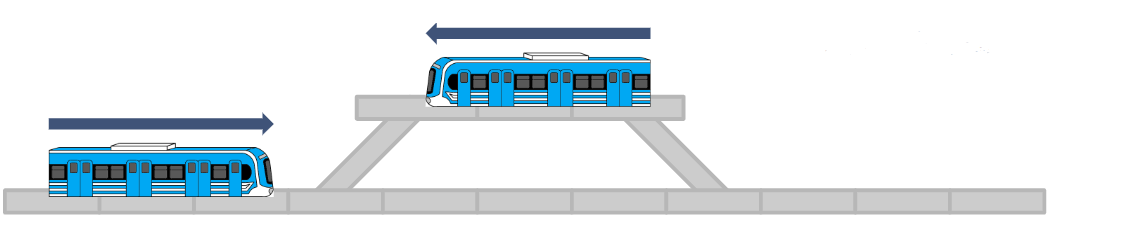
\includegraphics[width=1\textwidth]{Figuras/bypass}
		\centering\caption{Topología de derivación ferroviaria.}
		\label{fig:bypass_3}
	\end{figure}
	
	Es por eso que se decidió que la FPGA mediante la cual se implemente el sistema de enclavamiento debe recibir y transmitir la información a la cabina de señalamiento en formato serie. El uso de comunicación serie para la implementación del sistema es apropiado, ya que otros sistemas ferroviarios utilizan comunicación serie, como por ejemplo RS-485 o MVB en las redes de comunicación de trenes (TCN, del inglés \textit{Train Communication Network}) \cite{TCN}. La comunicación a implementar entre el sistema de enclavamiento y la cabina de señalamiento deberá ser flexible para ser utilizada en diferentes implementaciones con menor o mayor cantidad de elementos ferroviarios.
	
	En la Figura \ref{fig:GeneralCom} se presenta la propuesta de conexión de la FPGA con una computadora externa, que para el desarrollo y prueba de la solución hará las veces de la cabina de señalamiento. En la Figura \ref{fig:GeneralCom} también se representan los módulos internos de comunicación. La UART (del inglés \textit{Universal Asynchronous Receiver-Transmitter}), junto con las memorias FIFO (del inglés \textit{First-In First-Out}), se utilizan para implementar el intercambio de las tramas de datos entre la FPGA y la computadora.
	
	\begin{figure}[H]
		\centering
		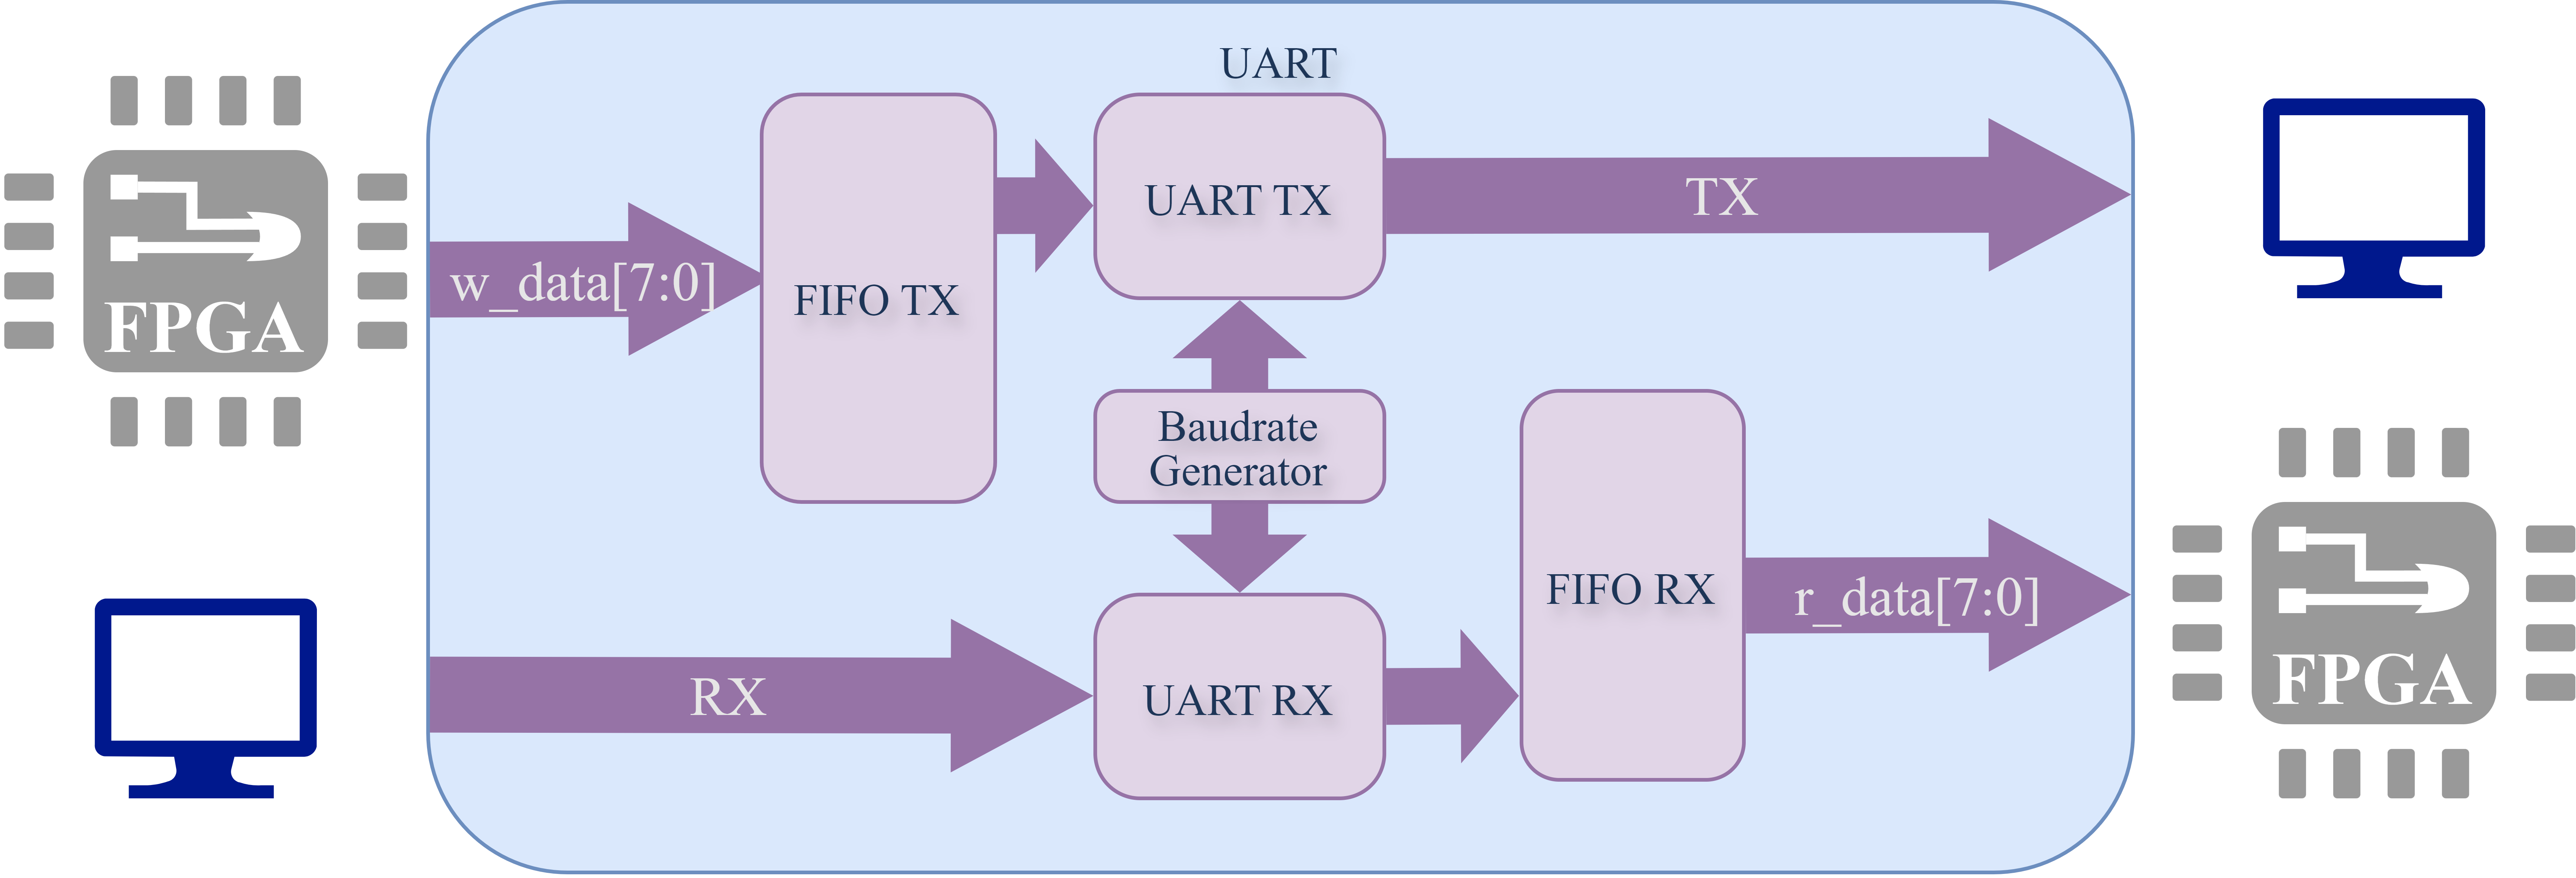
\includegraphics[width=0.7\textwidth]{Figuras/UART_module.png}
		\centering\caption{Conexión entre la FPGA y una computadora externa.}
		\label{fig:GeneralCom}
	\end{figure}
	
	El módulo de recepción (UART RX), que se ilustra en la Figura \ref{fig:GeneralCom}, es el encargado de procesar cada bit recibido con un baudrate preestablecido y almacenar cada bit en la FIFO RX. Al completarse un byte de datos, será enviado al sistema de enclavamientos, junto con una serie de pulsos para indicar cuándo deben ser leídos. El sistema de enclavamientos esperará a tener la cantidad de bytes necesarios (definidos por el ACG) para empezar a procesar la trama. Luego, el sistema de enclavamientos devolverá una nueva trama de bytes a la FIFO TX. Finalmente la nueva trama será enviada al módulo de transmisión (UART TX) que enviará la información bit a bit, con el mismo baudrate que fue recibido.
		
	En la Figura \ref{fig:Stream} se ilustra el formato definido para las tramas de entrada y salida. La trama tendrá un tamaño de entrada N y de salida M, con N igual que M. La cantidad de cada elemento ferroviario es definida por el RNA y el orden de los elementos es fijo y definido en el ACG. Los elementos que no existan en la locación analizada tendrán paquetes de datos de largo nulo. Además, la trama tendrá un caracter delimitador de entrada y de salida ($<$ y $>$ respectivamente). Todos los elementos de la trama serán hexadecimales en formato ASCII, para poder ser interpretados fácilmente en una terminal y ser menos susceptibles a errores por alteraciones en algún bit aleatorio.
	
	\begin{figure}[H]
		\centering
		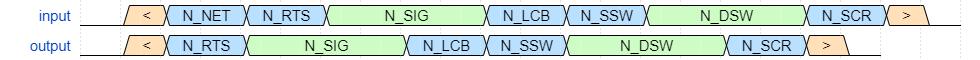
\includegraphics[width=1\textwidth]{Figuras/Tramas.png}
		\centering\caption{Tramas de datos y paquete de datos.}
		\label{fig:Stream}
	\end{figure}
	
	El largo de la trama de entrada y de salida queda definido por la Ecuación \ref{eq:StreamLength_in}. 
	
	\begin{equation} 
		\label{eq:StreamLength_in}
		\text{N} = 1\text{byte} (\text{N}_{NET}+\text{N}_{\text{RTS}}+\text{N}_{\text{LCB}}+\text{N}_{\text{SSW}}+\text{N}_{\text{SCR}}\text{N}_{\text{SIG}}+\text{N}_{\text{DSW}})
	\end{equation}
	
	Cada elemento dinámico requiere un sólo caractér hexadecimal para definir su estado utilizando sus 4 bits. Los 2 bits menos significativos definen el estado (\textit{STATE} en Figura \ref{fig:Stream}). Por ejemplo, la posición de un cambio de vías o el aspecto de una señal. Los 2 bits mas significativos definen el enclavamiento del elemento dinámico (\textit{LOCK} en la Figura \ref{fig:Stream}). El parámetro \textit{Lock} puede tomar tres valores: '00' para elementos disponibles, '01' para elementos que han sido reservados por una ruta pero aún no han sido enclavados y '10' para elementos enclavados.
	
	En la Figura \ref{fig:Stream_ejemplo1} se ilustran dos tramas recibidas en el caso de una topología ferroviaria que será explicada en profundidad en la Sección \ref{sec:ejemplo_1}.  La primer trama de datos representada el estado del sistema de enclavamiento cuando no se han solicitado rutas y la segunda ilustra una ruta pedida y habilitada. Ambas tramas cuentan con 11 netElements, 21 rutas, 23 señales, 2 pasos a nivel, 5 cambios de vías y los correspondientes tags iniciales y finales.
	
	En la primer trama se pueden apreciar: 11 secciones de vías sin ocupar (todos los valores en 1), 21 rutas sin solicitar (todos los valores en 0), 23 señales de las cuales podemos destacar 14 señales rojas (valores en 0), 4 señales naranjas (valores en 1), 3 señales amarillas (valores en 2) y 2 señales verdes (valores en 3). Además, la trama describe dos pasos a nivel con el brazo de barrera en alto (todos los valores en 1) y 5 cambios de vías, 3 de ellos en posición normal (valores en 0) y 2 en posición reversa (valores en 1). Debido que no existen rutas solicitadas ni habilitadas en esta trama (todos los valores en 0), todos los elementos tienen sus valores de LOCK en '00', lo que indica que se encuentran disponibles para ser enclavados por la ruta correspondiente.
	
	\begin{figure}[H]
		\centering
		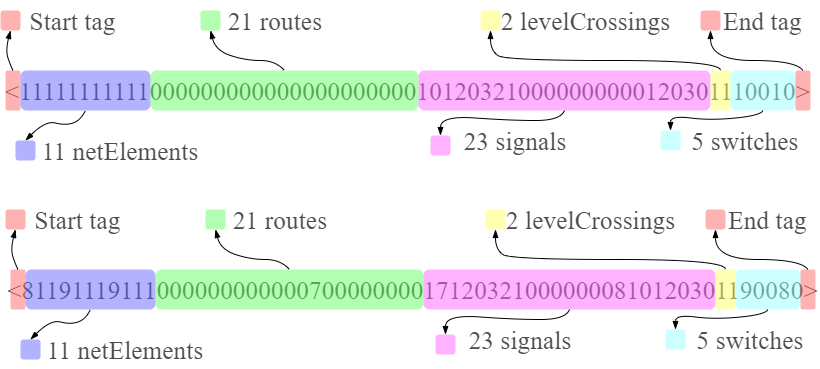
\includegraphics[width=1\textwidth]{Figuras/Trama_ejemplo.png}
		\centering\caption{Tramas de datos y paquete de datos.}
		\label{fig:Stream_ejemplo1}
	\end{figure}

	En la segunda trama, en cambio, se puede apreciar que el primer netElement (ne1) es representado con un 8 (1000), lo cual significa que se encuentra enclavado (10) y ocupado (00). Los netElements ne9 y ne15 son representados con un 9 (1001), ya que también se encuentran enclavados (10), pero no han sido ocupados (01). Además, la ruta 12 es representada con un 7 (0111), el estado de liberación secuencial (que será explicado en la Sección \ref{sec:ACG_rts}). Los semáforos que presentan valores superiores a 4 (0100) son aquellos que se encuentran reservados y los que presentan valores superiores a 8 (1000) se encuentran enclavados. En este caso, el semáforo S22 se representa con un 7 (0111, verde y reservado) y el semáforo T05 se representa con un 8 (1000, rojo y enclavado). Finalmente, los cambios de vías pares se encuentran en posición normal y los impares en posición reversa. En el caso del cambio de vías sw04, el valor 9 representa un cambio de vías enclavado en posición reversa y el cambio de vías sw07, el valor 8 representa un cambio de vías enclavado en posición normal.
	
	La implementación de los módulos de transmisión y recepción de la UART es invariante para cada locación, es decir, los recursos asignados serán los mismos, cualquiera sea el tamaño del sistema a implementar. Los módulos de memorias FIFO, en cambio, dependen de las características y del tamaño del sistema. Locaciones mas complejas tendrán valores de N y M mayores y, por lo tanto, requerirán FIFOs mas grandes. 
	
	
	
	
	%11111111111000000000000000000000101203210000000000120301110010
    %81191119111000000000000700000000171203210000000810120301190080
	
	
	%Con este criterio de diseño, en todos los demás casos, la FIFO de salida tendrá el mismo tamaño que la FIFO de entrada o a lo sumo será 50 \% menor, lo que representa un ahorro de 25 \% de los recursos estimados. Por ejemplo, si se necesita que la entrada tenga 15 bits y la salida 7 bits y se le asignara el mismo tamaño a ambas FIFOs; tanto la FIFO de entrada como la de salida necesitarán 16 bits cada una, dando un total de 32 bits. Pero si se aplica el criterio de tamaños desacoplados, entonces para la FIFO de salida podrían asignarse solamente 8 bits, dando un total de 24 bits, un 25 \% menos que los 32 bits que necesitaría si ambas FIFOs quedaran definidas según los datos de la entrada.